
\begin{figure}[H]
\centering
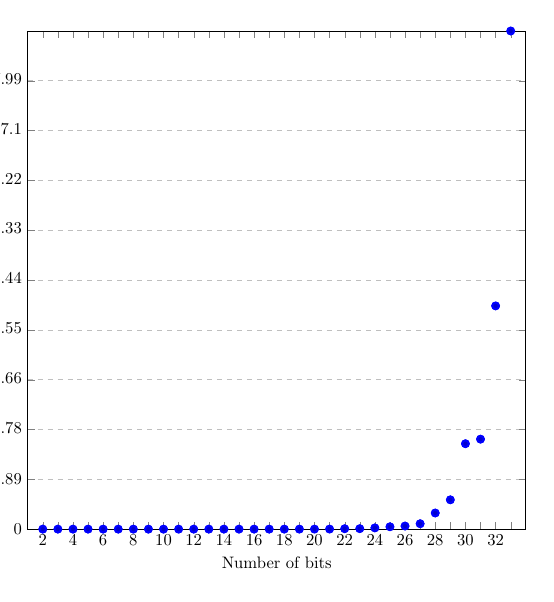
\begin{tikzpicture}[scale=0.6, trim axis left, trim axis right]
\begin{axis}[
    width=1\textwidth,
    height=1\textwidth,
    xlabel={Number of bits},
    ylabel={Time taken (s)},
    xmin=1.0, xmax=34.0,
    ymin=2.1e-05, ymax=9208.879762,
    xticklabels={2, , 4, , 6, , 8, , 10, , 12, , 14, , 16, , 18, , 20, , 22, , 24, , 26, , 28, , 30, , 32},
    xtick={2, 3, 4, 5, 6, 7, 8, 9, 10, 11, 12, 13, 14, 15, 16, 17, 18, 19, 20, 21, 22, 23, 24, 25, 26, 27, 28, 29, 30, 31, 32, 33},
    ytick={2.1e-05, 920.8879951, 1841.7759692, 2762.6639433, 3683.5519174, 4604.4398915, 5525.3278656, 6446.2158397, 7367.1038138, 8287.9917879},
    ymajorgrids=true,
    grid style=dashed,
]

\addplot+[
    blue,
    very thick,
    forget plot,
    only marks
    ]
    plot[
    very thick,
    error bars/.cd,
    y dir=plus,
    y explicit
    ]
    table[x=x,y=y,y error expr=\thisrow{y-max}] {
    x    y    y-max
    24	23.084672	0.0
25	43.861922	0.0
26	57.12664	0.0
27	100.000305	0.0
20	0.8914216	0.0062684
21	1.387053	0.000778
22	7.642371	0.0
23	8.677196	0.0
28	298.17366	0.0
29	541.862359	0.0
3	2.73e-05	1.7e-06
2	2.71e-05	3.79e-05
5	5.75e-05	1.45e-05
4	4.21e-05	9e-07
7	0.0001351	1.99e-05
6	7.36e-05	4e-07
9	0.0004602	1.48e-05
8	0.0002041	2.09e-05
11	0.0011537	1.33e-05
10	0.0008289	2.81e-05
13	0.0086567	7.13e-05
12	0.0055568	5.82e-05
15	0.0260357	0.0001113
14	0.0146861	9.49e-05
17	0.1003891	0.0016879
16	0.0652086	0.0077854
33	9208.879762	0.0
32	4126.774185	0.0
31	1663.577217	0.0
30	1579.287302	0.0
19	0.5951923	0.0088747
18	0.410265	0.049193

    };

\addplot+[
    blue,
    very thick,
    forget plot,
    only marks
    ]
    plot[
    very thick,
    error bars/.cd,
    y dir=plus,
    y explicit
    ]
    table[x=x,y=y,y error expr=\thisrow{y-min}] {
    x    y    y-min
    24	23.084672	0.0
25	43.861922	0.0
26	57.12664	0.0
27	100.000305	0.0
20	0.8914216	-0.0027956
21	1.387053	-0.000778
22	7.642371	0.0
23	8.677196	0.0
28	298.17366	0.0
29	541.862359	0.0
3	2.73e-05	-3e-07
2	2.71e-05	-6.1e-06
5	5.75e-05	-2.5e-06
4	4.21e-05	-1e-07
7	0.0001351	-3.1e-06
6	7.36e-05	-6e-07
9	0.0004602	-6.2e-06
8	0.0002041	-5.1e-06
11	0.0011537	-1.27e-05
10	0.0008289	-6.9e-06
13	0.0086567	-0.0001067
12	0.0055568	-6.08e-05
15	0.0260357	-5.07e-05
14	0.0146861	-0.0001031
17	0.1003891	-0.0004721
16	0.0652086	-0.0019066
33	9208.879762	0.0
32	4126.774185	0.0
31	1663.577217	0.0
30	1579.287302	0.0
19	0.5951923	-0.0025543
18	0.410265	-0.012257

    };

\end{axis}
\end{tikzpicture}
\vspace{-0.3cm}
\caption{Factors between 2 and 31 bits, modified agorithm}\label{fig:TrialDivisionGrowingprimes(modified:True)bits}
\end{figure}

